\subsection{EG-FET modeling}
\label{sec:EGFET_model}

When discussing EG-FETs, device modeling focuses on understanding the electrochemical and electrostatic processes occurring within these devices. As previously described in Section \ref{sec:EGFET}, EG-FETs consist of a semiconductor channel that is controlled by a gate electrode, separated by an electrolyte layer.

Given this, models of EG-FETs need to describe the charge transport in the semiconductor and electrolyte, their local variations in concentration, and the variations of the electrostatic potential on the device surface. To this end, the model analyzed in this thesis is based on the Nernst-Planck-Poisson equations, which account for all the mechanisms described above. In particular, the transport of holes in the semiconductor is governed by the drift-diffusion equation \eqref{eq:drift_el}, the changes in hole concentration over time are described by the continuity equation \eqref{eq:continuity_el}, and the electrostatic potential of the system is calculated according to the Poisson equation \eqref{eq:poisson_el}, \citep{delavariNernst2021}.

\begin{equation}
    \label{eq:drift_el}
    J_p = -D_p\left(\nabla p + fp\nabla V \right),
\end{equation}

\begin{equation}
    \label{eq:continuity_el}
    \nabla J_p = -\dfrac{dp}{dt},
\end{equation}

\begin{equation}
    \label{eq:poisson_el}
    -\dfrac{\varepsilon\nabla^2V}{F} = p,
\end{equation}

where $J_p$ is the flux of holes, $D_p$ is the diffusion coefficient of holes, $f=\frac{F}{RT}$ ($F$ is the Faraday's constant, $R$ is the ideal gas constant, $T$ is the temperature), $V$ is the electrostatic potential, $\varepsilon$ is the permittivity of the medium, and $p$ is the concentration of holes. \\
The same argument must be made for the transport of ions in the electrolyte:

\begin{equation}
    \label{eq:drift_ion}
    J_{c\pm} = -D_c\pm\left(\nabla c_{\pm} + fc_{\pm}\nabla V \right),
\end{equation}

\begin{equation}
    \label{eq:continuity_ion}
    \nabla J_{c\pm} = -\dfrac{dc_{\pm}}{dt},
\end{equation}

\begin{equation}
    \label{eq:poisson_ion}
    -\dfrac{\varepsilon\nabla^2V}{F} = c_+ - c_-,
\end{equation}

where $c_{\pm}$ and $D_c\pm$ represent the concentration and diffusion coefficient of ions, both positively ($+$) and negatively charged ($-$).

\begin{figure}[h]
    \centering
    \begin{minipage}{0.3\textwidth}
        \centering
        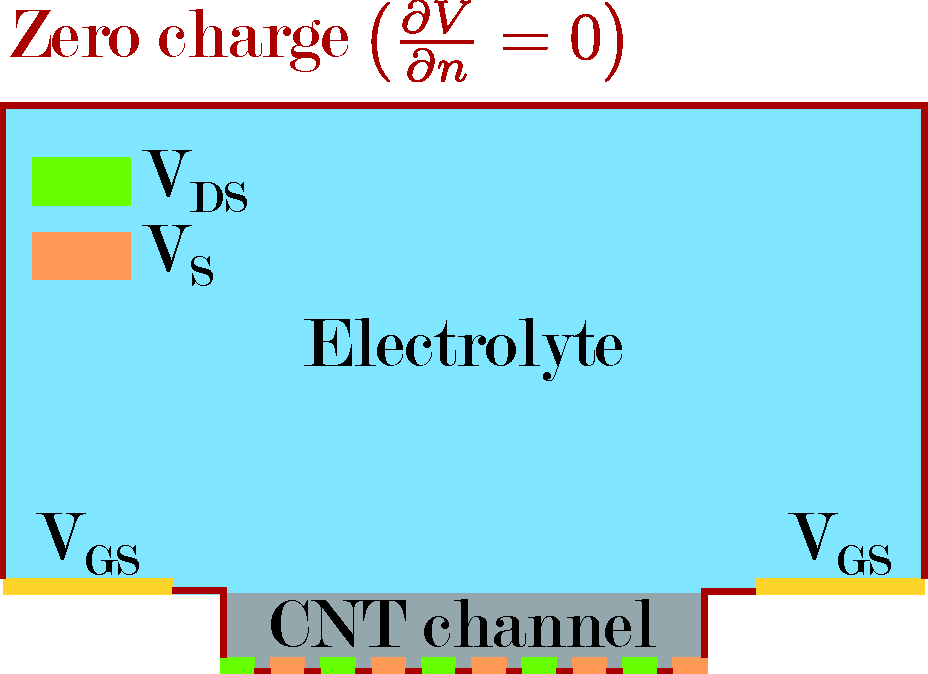
\includegraphics[width=\textwidth]{figures/chapter1/simulations/Fig7_boundaries1.pdf}
    \end{minipage}
    \hspace{10pt}
    \begin{minipage}{0.3\textwidth}
        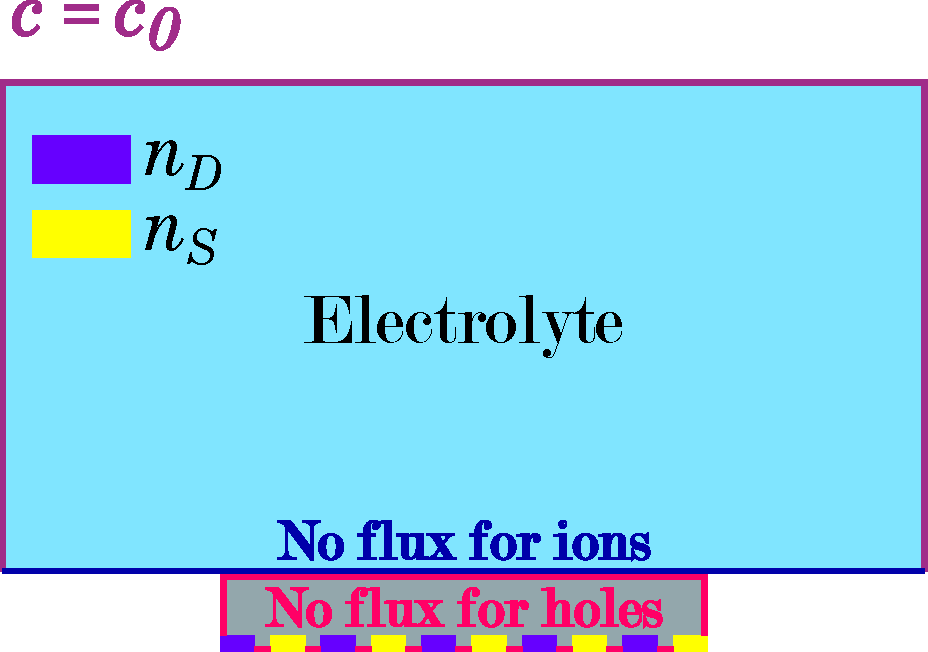
\includegraphics[width=\textwidth]{figures/chapter1/simulations/Fig7_boundaries2.pdf}
    \end{minipage}
    \caption{\note{Graphical representation of the boundary conditions as described in the text. The illustration highlights the constraints and parameters applied at the system's boundaries, which define the physical or mathematical behavior of the model.}}
    \label{fig:boundaryConditions}
\end{figure}

In order to solve the partial differential equations above, it is necessary to establish some boundary conditions. These boundary conditions specify the constraints or values that the solution must satisfy at the boundaries of the domain under consideration. They ensure that the problem is well-posed and enable the computation of an existing and physically meaningful solution. Without these constraints, the equations cannot be solved uniquely, as multiple or infinite solutions may satisfy the governing equations.

In the case of EG-FETs, the following boundary conditions must be established: the source is grounded, \ie{} $\mathrm{V_S} =$ \SI{0}{V}, while the gate and the drain have the voltages $\mathrm{V_G}$ and $\mathrm{V_D}$, respectively, whose values are assigned on the basis of the experiments carried out and which vary according to the type of simulation conducted. Outside the electrodes, the electric potential is zero:
%
\begin{displaymath}
    \dfrac{\partial V}{\partial N} = 0.
\end{displaymath}

Since there is no penetration of charges from the electrolyte to the semiconductor and vice versa, it is necessary to indicate the absence of hole and ion flux at the interface between the two materials. The concentration of holes at the source and drain must also be included among the boundary conditions as follows:
%
\begin{equation}
    n_S = n_0; n_D = n_S \exp\left(-\dfrac{eV_{DS}}{k_BT}\right),
\end{equation}

where $n_0$ is a constant indicating the initial concentration of holes at the source, $V_{DS}$ is the drain voltage, $e$ is the elementary charge, $k_B$ is the Boltzmann constant, and $T$ is the temperature; this condition thus takes into account the voltage that is applied between source and drain and updates the concentration of holes on the electrodes accordingly. For more clarity, please refer to Figure \ref{fig:boundaryConditions}

For EG-FETs, it is important to consider that during operation (and consequently during simulations), charges move and generate two EDLs at the interface between the semiconductor and the electrolyte, and between the gate and the electrolyte. In Section~\ref{sec:EGFET}, it was described that the EDLs work as two parallel plates of a capacitor, whose specific capacitance is described by the Helmholtz equation \citep{kimElectrolyteGated2013}:
%
\begin{equation}
    c = \dfrac{k\varepsilon_0}{\lambda_D},
\end{equation}

where $k$ is the relative permittivity of the electrolyte, $\varepsilon_0$ is the vacuum permittivity, and $\lambda_D$ is the Debye length. The latter is the quantity that describes the distance within an electrolyte over which the electric field generated by charges is screened by opposite charges present in the medium. In practical terms, it is the distance between the interface (both electrolyte-gate and electrolyte-semiconductor channel) and the outermost layer of ions, beyond which the surface charge has no effect \citep{nakatsukaAptamer2018}. The Debye length depends on various factors, such as temperature, ion density, and ionic strength (\ie{}, the salt concentration in the solution), and is defined as follows \citep{shkodraElectrolytegated2021}:
\begin{equation}
    \lambda_D = \sqrt{\dfrac{\varepsilon_r \varepsilon_0 k_B T}{2N_Aq^2I}},
\end{equation}

where $\varepsilon_0$ is the permittivity of free space, $\varepsilon_r$ is the relative permittivity of the medium, $k_B$ is the Boltzmann constant, $T$ is the temperature, $N_A$ is Avogadro's number, $q$ is the elementary charge, and $I$ is the ionic strength of the electrolyte.

Depending on the electrolyte used, the diffusion coefficient $D_p$ and the mobility of the charges $\mu_p$ may also vary, influencing how the charges move within the medium. These two quantities are related to each other by the Nernst-Einstein relation, formulated as follows \citep{delavariNernst2021}:
%
\begin{equation}
    \mu_p = \dfrac{D_p}{RT}.
\end{equation}
%
Once the movement of the charges within the electrolyte is understood, it is also necessary to account for the electric field applied to the field-effect transistor, which also influences the movement of the charges. To describe these movements, the Poole-Frenkel model is used \citep{gillDrift1972,delavariNernst2021}:
%
\begin{equation}
    \mu = \mu_p\exp\left(\dfrac{\gamma \sqrt{E}}{k_BT}\right),
\end{equation}
%
where $\gamma$ is the Poole-Frenkel constant, and $E$ is the electric field, given by $E = \frac{V_{DS}}{d_{SD}}$. This shows how the mobility $\mu$ depends on the applied $V_{DS}$ and the distance between the source and drain.

Having defined the operating mechanism of field-effect transistors, the next step is to evaluate their performance, that is, to calculate the output current. To this end, it is important to remember that there are two operating modes that depend on the applied voltages \citep{shkodraElectrolytegated2021}:

\begin{itemize}
    \item When $\lvert V_{DS} \rvert < \lvert V_{GS} \rvert - V_{th}$, the EG-FET operates in the linear regime. In this case, the current is calculated as in Equation \eqref{eq:ids_lin}:
    \begin{equation}
        \label{eq:ids_lin}
        I_{DS,lin} = \mu C_{EDL}\,\frac{W}{L}\left(V_{GS}-V_{th}\right)V_{DS}
    \end{equation}
    \item When $\lvert V_{DS} \rvert > \lvert V_{GS} \rvert - V_{th}$, the EG-FET is said to operate in the saturation regime. In this case, the current is calculated differently, as indicated in Equation \eqref{eq:ids_sat}:
    \begin{equation}
        \label{eq:ids_sat}
        I_{DS,sat} = \mu C_{EDL}\,\frac{W}{2L}\left(V_{GS}-V_{th}\right)^2
    \end{equation}
\end{itemize}
%
In the case of modeling EG-FETs and in the simulations performed, the calculation of \ids{} for the evaluation of the device performance was carried out differently; in fact, the current can be calculated by integrating the hole flux $J_p$ along the length of the channel, as shown in equation \eqref{eq:ids_int} \citep{newmanElectrochemical2021, chennitInkjetPrinted2023}:
%
\begin{equation}
    \label{eq:ids_int}
    I_{DS} = W \int_{0}^{l}J_p dl
 \end{equation}
%
In addition to the drain current equations, an important parameter to evaluate the performance of EG-FETs is the transconductance ($g_m$), which quantifies the amount of current in output relative to changes in the input voltage $\left(\frac{I_{out}}{V_{in}} \right)$. For EG-FETs, it is defined as:
%
\begin{equation}
    \label{eq:transconductance}
    g_m = \mu C_{\text{ox}} \frac{W}{L} (V_{GS} - V_{th}),
\end{equation}
%
where $C_{\text{ox}}$ is the oxide capacitance per unit gate area, $W$ is the channel width, and $L$ is the channel length. This equation indicates well how the transconductance depends on both material properties and device geometry, thus influencing the sensitivity and signal amplification in sensing applications.